\documentclass[a4paper,utf8,11pt, onecolumn]{ctexart}
\usepackage{amsmath}
\usepackage{amssymb}
\usepackage{array}
\usepackage{siunitx}
\usepackage{natbib}
\usepackage{subcaption}
\usepackage{fancyhdr}
\usepackage{graphicx}
\usepackage{authblk}
\newcommand{\RN}[1]{%
  \textup{\uppercase\expandafter{\romannumeral#1}}%
}
\renewcommand{\captionfont}{\kaishu\zihao{5}}
\renewcommand{\captionlabelfont}{\kaishu\zihao{5}}
\providecommand{\keywords}[1]{\textbf{关键字:} #1}
\addtolength{\topmargin}{-54pt}
\setlength{\oddsidemargin}{-0.9cm}  % 3.17cm - 1 inch
\setlength{\evensidemargin}{\oddsidemargin}
\setlength{\textwidth}{17.00cm}
\setlength{\textheight}{24.00cm}    % 24.62
\renewcommand{\baselinestretch}{1.1} %定义行间距

\title{\huge{健壮的实时面部识别系统}}
\author[1]{PAUL VIOLA\thanks{viola@microsoft.com}}
\author[2]{MICHAEL J. JONES\thanks{mjones@merl.com}}
\affil[1]{Microsoft Research, One Microsoft Way, Redmond, WA 98052, USA}
\affil[2]{Mitsubishi Electric Research Laboratory, 201 Broadway, Cambridge, MA 02139, USA}
\date{}
\begin{document}
\bibliographystyle{plainnat}
\maketitle
\begin{abstract}
\noindent 这篇论文描述了一个人脸识别系统. 它能够在以高检测率快速处理图像. 这个系统主要有三个主要贡献.
第一, 我们引入了``积分图''这一新的图像表现形式. 利用它我们能够快速计算出检测器需要的图像特征.
第二, 使用 AdaBoost 学习算法\citep{freund1995desicion}构建出简单高效的分类器. 它能在非常大的潜在特征集合中选取少量重要可视化特征. 
第三, 我们采用级联分类器的方法快速去除图像的背景, 将更多的计算投入到识别面部特征上. 
我们已经在面部识别领域进行了一系列的实验. 和之前最好的系统 \citep{sung1998example, rowley1998neural,schneiderman2000statistical,yang2000snow} 相比, 这个系统在面部识别的表现上略逊一筹. 在传统电脑上的实现面部识别速率能够达到每秒$15$帧. \\

\keywords{面部识别, 加速, 人类感知}
\end{abstract}
\section{引言}
这篇论文使用新的算法和观点构建了一个健壮快速的视觉识别系统. 在这个基础上, 我们已经完成一个正脸识别系统. 它在识别率和误报率上已经达到了之前发布的最好结果 \citep{sung1998example, rowley1998neural,osuna1997training,schneiderman2000statistical,yang2000snow}. 
不同于之前的那些, 这个系统能够非常快速地识别人脸. 在$384\times288$像素的图像以及700 MHz,  Intel Pentium \RN{3}的传统电脑上, 识别速率达到了每秒$15$帧. 
其他的面部识别系统使用了多个辅助信息来达到极高的速度, 例如视频序列中的图像差异以及图片中像素的颜色. 而我们的系统仅仅使用了单张灰度图像中的信息. 那些辅助信息仍然能够帮助我们达到更高的帧速. 
我们的面部识别系统主要有三个贡献. 下文将对它们进行简短介绍. 在其他章节中我们将详细描述. 
这篇论文的第一个贡献是``积分图''这一新型图像表现形式. 它能够帮助我们快速地进行特征计算. 受到\citet{papageorgiou1998general}的工作的启发, 我们的检测系统不直接工作在图像明暗度上. 
和之前的作者一样, 我们采用类似于哈尔基函数的一个特征集合. 我们也使用比哈尔基过滤更加复杂的过滤方式. 为了能够在多个尺寸上快速计算图像特征, 我们引入了积分图. 它非常类似于计算机图形学中纹理贴图采用的积分图\citep{crow1984summed}. 
我们只要对图像中每个像素进行若干操作便能计算出其积分图. 一旦计算出积分图, 我们便能在常数时间内计算出任何尺寸任何地方的类哈尔特征. 

这篇论文的第二个贡献是实现了一个简单高效的分类器. 该分类器采用 AdaBoost 算法\citep{freund1995desicion}, 能够从大量的潜在特征集合中选择少量重要特征. 在图像的任何子区域内类哈尔特征的数量远远超过了像素的数量. 
为了保证分类速度, 学习过程中我们必须去掉非常多的特征, 将精力集中在小部分重要特征上. 受到\citet{tieu2000boosting}的启发, 我们通过采用 AdaBoost 算法将每一个弱分类器限制到单一特征. 最终在算法增长过程中的每个阶段, 弱分类器的选择过程就可以看作是特征的选择过程. AdaBoost 既提供了高效算法, 也强有力地保证了一般情况下的性能\citep{schapire1998boosting}. 

这篇论文的第三个主要贡献是提供了将更多分类器连接成级联结构的一种方法. 它通过关注图像的可行区域极大地提高了检测速度. 这个想法来源于如下论断:快速判断人脸将出现在图像的哪一部分通常是可行的
\citep{tsotsos1995modeling,itti1998model,amit1999computational,fleuret2001coarse}. 
只有那些可行区域才值得进行更多复杂的处理流程. 一个关键参数是检测过程的漏报率. 检测器必须能够识别出几乎所有的人脸. 

我们将描述训练一个简单高效的分类器流程, 它将用于监督式的认知器训练中\footnote{称之为监督式的是因为认知器被训练为识别特定类别的样本}. 第一层检测器在很大的数据集上可以达到过滤$50\%$图像并保留$99\%$面部区域的最终效果. 
这个过滤器也是非常高效的. 它能在图像的每个地方只执行$20$次操作, 总计大约$60$个微处理器指令. 

那些没有被最初的分类器拒绝的区域将被接下去的一系列分类器处理, 每一个都将比前一个略微得复杂一点. 如果其中一个区域被某个分类器拒绝, 那么它便不会再被继续处理. 这个级联检测流程的结构就是一个蜕化决策树, 这个工作和\citet{fleuret2001coarse}的工作以及\citet{amit1999computational}的工作有关. 

一个完整的面部识别级联结构有$38$个分类器, 将近$80000$个操作. 这个级联结构仍然能达到非常快的平均检测速度. 在一个困难的数据集上, 其中包含$507$张脸, $75000000$个子区域, 识别的过程中平均每一个子区域使用了$270$个微处理器指令. 作为对比, 这个系统比\citet{rowley1998neural}实现的识别系统快了将近$15$倍\footnote{Henry Rowley 非常慷慨地将他的系统实现给我们用于直接的比较. 最终报告的结果是根据它最快的系统作出. 虽然很难从公布的论文中看出, Rowley-Baluja-Kanade 的检测器已经被公认为是最快的检测系统, 且经受了很多实际问题的考验}. 

一个极端快速的人脸识别器有着广阔的应用前景, 包括人机交互接口, 图像数据库以及电视会议. 速度上的提升将使那些实时的面部识别应用系统成为可能. 在那些不需要高帧速的应用中, 重要的后期处理和分析也将变得可行. 
另外, 我们的系统能够在大量小功率设备上实现, 比如手持设备以及嵌入式处理器等. 在实验室中, 我们在一台小功率 200mips Strong Arm 处理器上实现了这个面部识别系统. 这个处理器没有浮点运算硬件, 但是我们的系统仍然达到了每秒两帧的速度. 
\subsection{概述}
论文接下去的章节将讨论检测器的实现, 相关的理论以及实验. 
章节\ref{sec:feature}将详细描述特征的形式以及快速计算的方法. 章节\ref{sec:learning}将讨论将这些特征结合在一起形成分类器的方法. 作为 AdaBoost 算法的一个应用, 机器学习也表现为特征选取机制. 尽管用这种方式完成的分类器有着良好的计算和分类性能, 但是作为实时分类器, 它们还是不够快. 
章节\ref{sec:cascade}将描述级联分类器的方法. 最终形成一个快速高效的面部识别器. 章节\ref{sec:result}将详述多个测试结果以及我们采取的实验方法. 最后, 章节\ref{sec:discussion}对这个系统和其他相关系统之间关系进行了讨论. 
\section{特征}\label{sec:feature}
我们的面部识别过程利用简单特征的值分类图像. 使用特征而不是直接用像素有着很多的优势. 最为常见的一点就是能够编码用有限的训练集很难学习的局部领域知识. 对于这个系统, 还有另外一点优势:基于特征的系统比基于像素的系统运行得更快. 

这种简单特征令人想起\citet{papageorgiou1998general}中使用的哈尔基函数. 更专业地说, 我们使用了三种特征. 2-矩形特征的值是两个矩形区域像素和的差. 这两个区域有相同的大小和形状, 并且水平或者竖直相邻.
一个 3-矩形特征由两边矩形的和减去中间矩形的和而得. 最后一个 4-矩形特征由对角矩形和之差求得.(图\ref{fig:rectangle})
\begin{figure}[!htb]
\centering
\begin{subfigure}{0.3\textwidth}
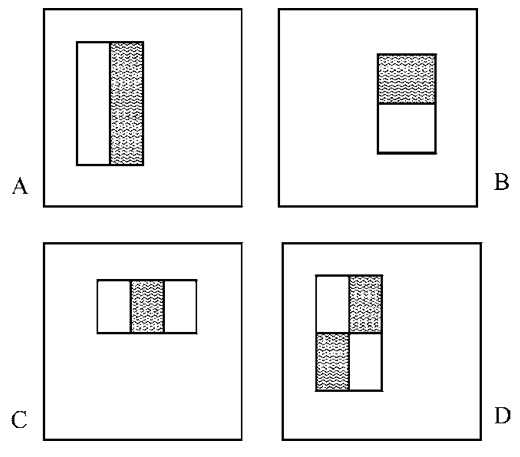
\includegraphics[width=\textwidth]{rectangle.png}
\renewcommand{\captionlabelfont}{\kaishu\zihao{6}}
\caption{\zihao{6} 在检测区域内部的矩形特征. 灰色区域的像素和减去白色区域的像素和. (A) 和 (B) 是 2-矩形特征, (C) 是 3-矩形特征, (D) 是 4-矩形特征}
\label{fig:rectangle}
\end{subfigure}
\quad\quad\quad\quad
\begin{subfigure}{0.3\textwidth}
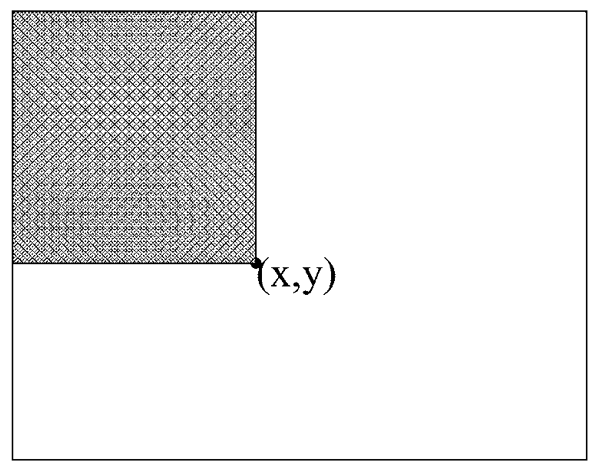
\includegraphics[width=\textwidth]{int.png}
\renewcommand{\captionlabelfont}{\kaishu\zihao{6}}
\caption{\zihao{6}$(x,y)$处的积分值是其左上角所有像素之和}
\label{fig:int}
\end{subfigure}
\caption{矩形特征和积分图的计算}
\end{figure}

假设检测器的初始分辨率为 $24\times24$, 矩形特征的整个集合大小为$160000$. 注意到这个集合不像哈尔基, 是过完备的\footnote{一个完备基各基本元素之间是线性独立的, 在图像空间中有相同数量的元素. 在$576$这个例子中, $160000$个特征的集合是完备基的很多倍}.

\subsection{积分图}
利用我们引入的图像中间表现形式---积分图\footnote{在图像领域中这和``求和表''比较类似\citep{crow1984summed}. 我们在这里选择一个不一样的名称, 强调它用于图像分析中而不是纹理映射}, 矩形特征能够极快地计算出来. 在$(x, y)$处的积分图包含了在该点左上方像素点的和, 用公式来说就是:
\[
    ii(x, y)= \sum_{x'\leq x, y'\leq y} i(x', y')
\]

其中 $ii(x, y)$ 表示积分图, 而 $i(x, y)$ 表示原始图(图\ref{fig:int}). 使用如下的递归式:
\[
    \begin{array}{r@{}>{{}}l@{\qquad}r@{}>{{}}l}
        s(x,y)&=s(x,y-1)+i(x,y)\\
        ii(x,y)&=ii(x-1,y)+s(x,y)
    \end{array}
\]

其中 $s(x, y)$ 表示行的累和, 初始条件为$s(x,-1)=0, ii(-1,y)=0$. 只要遍历一遍整张图, 积分图便能计算出来. 

通过积分图, 任何矩形和可以通过四个数组查询计算出来(图\ref{fig:feature_calculate}). 很显然, 两个矩形的差值能够通过八个查询计算出来. 既然 2-矩形特征通过相邻的矩形定义, 它便能用六个数组查询计算出来, 同理 3-矩形特征用了八个数组查询, 4-矩形特征用了九个数组查询.

积分图的另一个来源是\citet{simard1999boxlets}的工作. 其中作者指出在线性运算中 (例如 $f\ast g$), 任何可逆线性运算可以施加于$f$或$g$上, 只要其逆运算一同施加于线性运算的结果之上. 例如在图像的卷积中, 如果微分运算施加于图形其卷积核上, 那么卷积结果必须通过二重积分运算才能和原式相等:
\[
    f\ast g = \iint(f'\ast g')
\]
若$f$和$g$的微分结果是稀疏的或者能够让它变得稀疏, 那么卷积的速度便能大大加快. 另外一个相似的观点就是线性运算和其逆运算分别施加于$f$和$g$上, 结果仍然不变:
\[
    (f'')\ast\iint g = f\ast g
\]
在我们系统中采用的矩形和的计算能够抽象为点积运算, $i\cdot r$, 其中$i$表示图像而$r$表示一个盒函数 (box car image, 感兴趣的矩形区域为$1$, 其他区域为$0$). 该运算又可写为:
\[
    i\cdot r = (\iint i)\cdot r''
\]
事实上该式中的双重积分就是我们算得的积分图 (先以行再以列). 第二个微分式表示在矩形四角的$\delta$函数. 等式右侧的点积运算就可以通过四个数组查询解决.
\begin{figure}[!t]
\centering
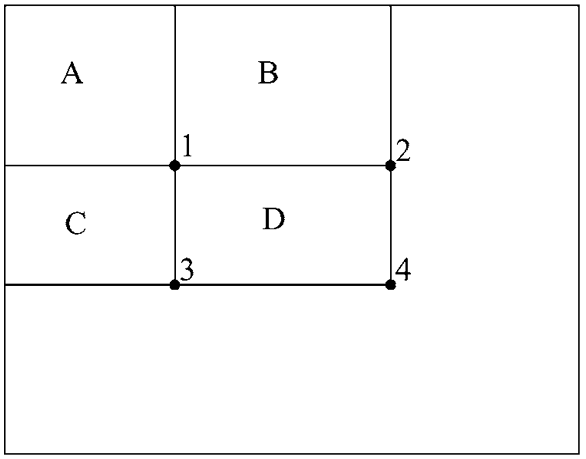
\includegraphics[width=0.4\textwidth]{feature_calculate.png}
\caption{矩形$D$的像素和可以通过四个数组查询计算. 如图$1$是矩形$A$的像素和, $2$是矩形$A+B$, $3$是矩形$A+C$, $4$是矩形$A+B+C+D$. $D$的和就是$4+1-(2+3)$}
\label{fig:feature_calculate}
\end{figure}

\subsection{特征讨论}
和方向可变滤波器\citep{freeman1991design,greenspan1994overcomplete}等其他过滤器相比, 我们的矩形特征在某种程度上是比较原始的. 方向可变滤波器以及其他类似的滤波器擅长于边界分析, 图像压缩以及纹理分析. 
尽管矩形区域对边界, 条状物以及其他简单的图形结构有着较好的敏感度, 但是也是十分粗糙的. 不像那些方向可变滤波器, 矩形区域只有水平, 垂直, 对角三种排列方式. 因为正交性不是这个特征集合主要考虑的问题, 我们生成了数量巨大而多样的矩形特征. 这个数量已经远远过完备, 超过了所需数量将近$400$倍.
这个过完备的集合有着任意的纵横比以及精细的采样位置. 特别地, 它是一个能够有效学习的丰富的图像表示形式. 另外, 矩形区域计算的高效性极大地弥补了它的缺陷. 

为了对积分图技术带来的计算优势体会得更加深刻, 考虑计算金字塔状变化的图像序列时所用的传统方法. 就像大多数的面部识别系统, 我们的检测器扫描了图像的多种尺寸大小. 从基本尺寸$24\times24$像素开始, 一张$384\times288$像素大小的图像扫描了$12$种尺寸, 每一种都比前面一种大$1.25$倍.
传统方法和这个类似, 不过每次的尺寸都比前一次小$1.25$倍. 一个固定尺寸的检测器扫描了其中的每一张图像. 然而直接计算这个序列太耗费时间. 在传统机器上采用双线性插值算法的高效实现, 计算$12$种尺寸仍然需要$0.05$秒 (Intel P\RN{3} 700MHz 处理器)\footnote{特殊硬件和指令集能够改变这个分析结果. 在传统的软件算法前提下进行性能的比较仍然是有指导意义的}.

然而, 我们定义了一个矩形特征集, 其中的每一个特征只需要一点点操作便能从任何尺寸和位置上计算出来. 我们将在第四章节讲述如何使用两个矩形特征构造高效的面部检测器. 归功于计算特征的高效, 这个面部识别程序能够以每秒$15$帧的速度用一个尺寸完整地扫描整张图像.

\section{学习分类函数}\label{sec:learning}
只要有一个特征集以及正例反例图组成的训练集, 任何机器学习的算法就可以用来学习分类函数. \citet{sung1998example}中用了一个高斯混合模型.\citet{rowley1998neural}使用了一小部分图像特征集合以及神经网络.\citet{osuna1997training-2}使用了一个支持向量机. 最近\citet{yang2000snow}公布了一个新型图像表现形式并使用了 Winnow 学习程序.

不得不提及的是和一个图片子区域相关的矩形特征有$160000$个之多, 远远超过了像素的数量. 即使每个特征都能十分高效地计算, 计算那么多特征也是不切实际的. 根据我们实验后的结论, 只有一小部分的特征可以作为有效的分类器. 问题就在于如何找到这些特征.

我们使用 AdaBoost 算法的一个变体选取特征并训练分类器\citep{freund1995desicion}. 最初, AdaBoost 算法被用来提高简单学习算法的分类性能, 例如用来加速一个简单的感知器. 它通过联合多个弱分类函数形成一个更加强大的分类器. 在这一方面, 弱学习算法被称为弱学习器.
举个例子, 感知器学习算法从多个感知器中选择分类错误率最低的一个. 因为即使是最好的分类器效果也不是很好, 甚至对于特定问题只能达到 $51\%$的正确率, 所以它被称为弱学习器.
为了提高弱学习器的性能, 一系列学习问题有待解决. 第一轮的学习过后, 为了强调出被先前的弱分类器错误分类的那些样本, 权值必须重新标注. 最终的强分类器由一系列受权重和阈值约束的弱分类器组成\footnote{弱学习器是一个感知器学习算法的情况下, 最终的增强分类器是一个两层的感知器. 原则上两层的感知器比任何一个单一感知器都要强}.

AdaBoost 学习算法强有力地保证了我们结果的正确性.\citet{schapire1997boosting}中证明强分类器的训练错误率随着训练轮数的增加以指数方式下降到$0$. 之后又出现了一些更加重要的成果. 其中的关键就是分类器的泛化性能和样本边界有关, 而 AdaBoost 算法能够很快达到那些边界.

传统的 AdaBoost 算法流程可以简单地视作贪心特征选取. 考虑一个一般性的问题. 很多分类函数通过加权多数表决的形式结合在一起, 那么如何将高权值分配给好的分类函数而将低权值分给差的分类函数呢? 
AdaBoost 算法有着一个良好的机制, 能够从低权值的分类器中选取一部分好分类器. 打个比方, 在弱分类器和特征之间, AdaBoost 算法能够高效地选取出一些好的特征, 可是好特征远不止这些.

完成这个类比的一个可行方法就是将弱学习器限制在只依赖单一特征的分类函数集中. 为了达到这个目标, 弱学习算法被设计成选取能够最优划分正反样本的单一矩形特征 (和\citet{tieu2000boosting}在图像数据库领域达到的成就相似). 学习算法对每一个特征最优化阈函数, 例如最小化误分类样本数量. 一个弱分类器 $h(x,f,p,\theta)$ 包含了特征函数$f$, 阈值$\theta$以及代表了不等式方向的$p$:
\[
    h(x,f,p,\theta) =
    \begin{cases}
        1 &\quad\text{if}\quad pf(x)<p\theta \\
        0 &\quad\text{otherwise}
    \end{cases}
\]
公式中$x$表示图像的$24\times24$像素大小的子区域.

实际上没有一个单一特征能够小错误完成分类任务. 在程序早期的特征选取中错误率在$0.1-0.3$之间. 在后期随着任务变得不断困难, 特征选取的错误率在$0.4-0.5$之间. 图\ref{fig:adaboost}展示了该学习算法.
\begin{figure}[htb]
\kaishu\zihao{5}
    \caption{一个能够在线查询学习的增强算法.$T$个假设使用单一特征构建. 最终的假设是$T$个假设的加权线性结合, 其中的权值和训练误差成反比}
    \label{fig:adaboost}
    \begin{itemize}
        \item 由$n$个样例图$(x_1,y_1),\ldots,(x_n,y_n), y_i=0, 1$分别表示反例和正例.
        \item 初始化权值 $w_{1,i}=\frac{1}{2m}, \frac{1}{2l},y_i=0,1$其中$m$和$l$分别是反例和正例的数量.
        \item 对于每一个$t=1,\ldots,T$:
            \begin{enumerate}
                \item 规范化权值$w_{t,i}\leftarrow \frac{w_{t,i}}{\sum_{j=1}^n w_{t,j}}$
                \item 根据加权误差大小选取最好的弱分类器
                    \[
                        \epsilon_t=\min_{f,p,\theta}\sum_i{w_i| h(x_i,f,p,\theta)-y_i |}.
                    \]
                    查看章节对高效实现的讨论
                \item 定义函数$h_t(x)=h(x,f_t,p_t,\theta_t)$, 其中$f_t,p_t,\theta_t$是满足上式最小化$\epsilon_t$后的值
                \item 更新权值
                    \[
                        w_{t+1,i}=w_{t,i}\beta_t^{1-e_i}
                    \]
                    其中$e_i=0$仅当$x_i$被正确分类, 否则$e_i=1$. $\beta_t=\frac{\epsilon_t}{1-\epsilon_t}$.
            \end{enumerate}
        \item 最终的强分类器为
            \[
                C(x)=
                \begin{cases}
                    1 &\quad\sum\limits_{t=1}\limits^T \alpha_t h_t(x)\geq \frac12\sum\limits_{t=1}\limits^T\alpha_t\\
                    0 &\quad\text{otherwise}
                \end{cases}
            \]
    \end{itemize}
\end{figure}

我们使用的弱分类器 (带有阈值的单一特征) 可以看作是单一节点的决策树. 像这样子的结构在机器学习中称为单层决策树.\citet{freund1995desicion}在最初也尝试过加速单层决策树.
\subsection{学习讨论}
在表中描述的算法用来从一组弱分类器中选取关键的弱分类器.尽管 AdaBoost 算法非常高效, 但是弱分类器的集合太大了. 一组特征/阈值对应着一个弱分类器, 若有$K$个特征以及$N$个样例, 则弱分类器就有$KN$个. 为了强调对$N$的依赖, 假设样例已经根据一个特定的特征值进行了排序. 考虑到训练过程, 被排序样例中相同对之间的阈值是等价的. 因此不同的阈值总数为$N$. 在一个$N=20000, K=160000$的任务中, 有$3.2\times 10^9$ 个弱分类器对.

这组方法也能够利用M个弱分类器学习出一个感知器\citep{john1994irrelevant}. 在每轮学习中, 这个方法将一个弱分类器添加至感知器中, 使得添加后的感知器错误率最低. 每轮训练的时间复杂度至少为$O(NKN)$ ($60$兆个操作). 每一轮中将遍历所有的特征对, 并用每一个特征评估每一个样例.
这个过程忽略了学习感知器权重的时间. 即使是这样, 学习$200$个特征的分类器的时间复杂度也大约是$O(MNKN)$, 差不多是$10^{16}$个操作.

作为特征选取算法, AdaBoost 的一个关键优势就在于学习速度. 使用 AdaBoost 算法后一个具有$200$个特征的分类器可以在$O(MNK)$的时间或者大约$10^{11}$个操作内学习得到. 另一个关键优势在于每一轮学习中对前一个选取的特征的依赖性已经高效而完整的隐含在样例权重中, 利用这些权重能够在常数时间内评估一个给定的弱分类器.

弱分类器的选取算法如下. 对于每一个特征, 样例根据该特征的值进行排序. AdaBoost 最优阈值便能在单次遍历中计算得到. 对于其中的每一个元素, 我们计算和维护四个和:
\begin{itemize}
\item 正样例权重之和$T^+$
\item 反样例权重之和$T^-$
\item 小于当前样例的正样例权重之和$S^+$
\item 小于当前样例的反样例权重之和$S^-$
\end{itemize}
在已排序列表中, 分割当前样例和之前样例产生的误差为:
\[
e=\min(S^++(T^--S^-),S^-+(T^+-S^+))
\]
将所有低于当前样本的标记为反样例, 将高于当前样本的标记为正样例, 或者相反. 取两种情况中的最小误差. 这些和在搜索的过程中很容易更新.

有很多的特征识别过程已经被提出 (参见\citet{webb1999statistical}的第八章节). 我们最终的应用采取了一个非常激进的过程, 大量的特征被丢弃. 在一个相似的识别问题中,\citet{papageorgiou1998general}基于特征差异
提出了一个特征选取的方法. 他们在总共 $1734$ 个特征中选取出$37$个特征, 取得了很好的结果. 尽管这已经是一个极大的简化措施, 但是对于每一个图像子区域待评估的特征数量还是太多.

\citet{yang2000snow}基于 Winnow 指数感知器学习规则提出了一个特征选取过程. 他们使用了一个大而不同寻常的特征集合, 其中每个像素和一个$d$维二进制向量关联 (一个像素有值$x\in[0, d-1]$, 与之对应的向量第$x$维置为$1$, 其他为$0$). $n$个像素对应的二进制向量可以组成和一个$nd$维的二进制向量. 分类器就是一个对输入向量不同维分配不同权重的感知器. Winnow 学习过程收敛到一个结果, 其中大部分权重都是$0$, 然而仍然保留了很多特征 (可能是几百或者几千).

\subsection{学习结果}
尽管更多训练和性能的细节将在章节\ref{sec:result}展示, 一些简单的结果值得在这里讨论. 最初的实验说明由$200$个特征训练出来的分类器能得到合理的结果 (图\ref{fig:f2}). 在有$95\%$检测率的同时, 该分类器测试集中的误报率保持在$1/14084$的水平.
\begin{figure}
\center
\begin{subfigure}{0.3\textwidth}
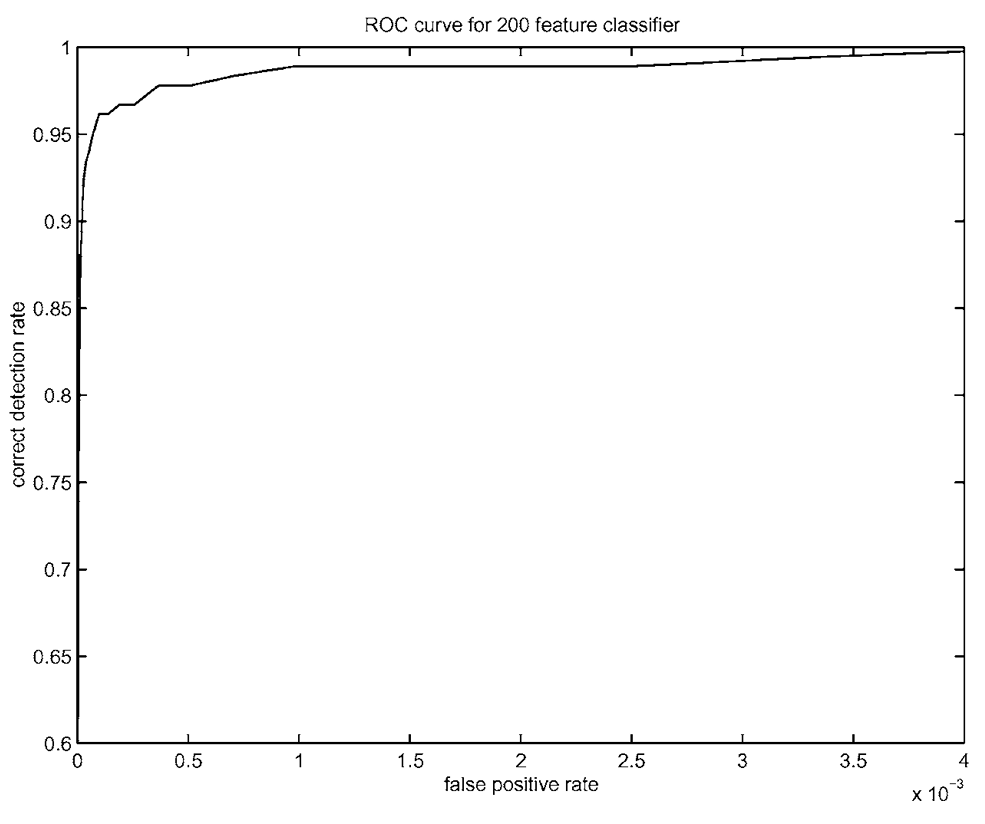
\includegraphics[width=\textwidth]{200.png}
\renewcommand{\captionlabelfont}{\kaishu\zihao{6}}
\caption{\zihao{6}具有$200$个特征的分类器的 ROC 曲线}
\label{fig:f2}
\end{subfigure}
\quad\quad\quad\quad
\begin{subfigure}{0.3\textwidth}
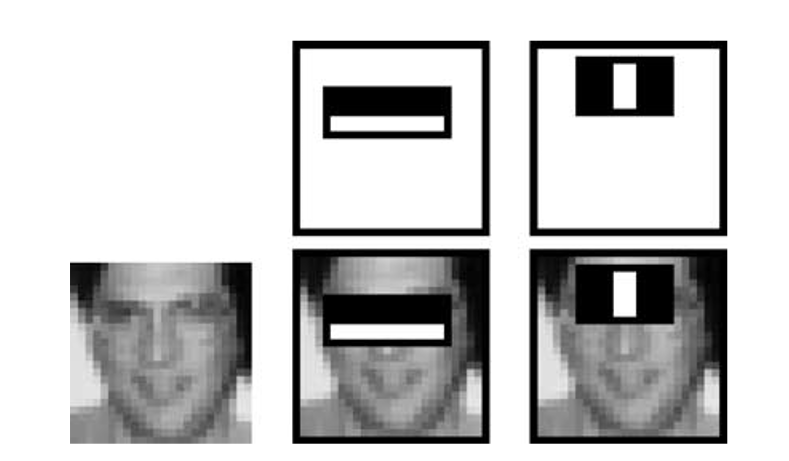
\includegraphics[width=\textwidth]{eye.png}
\renewcommand{\captionlabelfont}{\kaishu\zihao{6}}
\caption{\zihao{6}AdaBoost 选取的第一和第二个特征. 第一行展示了两个特征, 第二行将特征覆盖在了训练的人脸上. 第一个特征展现了上脸颊和眼部的亮度差异, 充分利用了眼部比脸颊黑的特点. 第二个特征比较了眼部和鼻梁的亮度差异.}
\label{fig:eye}
\end{subfigure}
\caption{}
\end{figure}
这个结果是令人振奋的, 但是作为在真实应用中使用的面部检测器, 误报率必须要接近$1/1000000$才可以.

在面部检测任务中, AdaBoost 算法开始选取的矩阵特征是有意义的并且容易被解释. 它选取的第一个特征看上去聚焦于如下性质: 眼部区域常常比鼻子和脸部区域更黑 (图\ref{fig:eye}). 和检测的子区域相比, 这个特征相对来说比较大, 而且对面部大小和位置不敏感. 选取的第二个特征着重于眼部比鼻梁更黑这个特征.

综上所述, $200$个特征的分类器初步证明了一个由矩形区域构造出的增强分类器是一个高效的面部检测技术. 在检测方面, 这些结果是迷人的, 但是对于实际任务来说还是不够. 在计算方面, 这个分类器非常快, 扫描一个$384\times288$像素的图像只需要$0.7$秒. 不幸的是, 向分类器添加特征这一提高性能的最直接的技术增加了非常多的计算时间.

\section{引人注目的级联结构}\label{sec:cascade}
这个章节描述了构建级联分类器的一个算法. 它能提高检测性能并大幅度减少计算的时间. 其中的关键想法就是能够通过构建更小更高效的增强分类器拒绝很多负的子区域, 检测出几乎所有的正例. 比较简单的分类器被用来拒绝大量子区域, 之后调用更复杂的分类器来减少误报率.

我们通过使用 AdaBoost 算法训练分类器构建出级联层级结构. 从一个 2-特征强分类器开始, 我们通过调整强分类器的阈值减小漏报率的方式得到一个高效的面部过滤器. 起初的 AdaBoost 阈值$\frac12\sum_{t=1}^T\alpha_t$被设计成能够在训练集上得到一个较低的错误率. 一个较低的阈值带来了较高的检测率和较高的误报率. 基于在验证集上的性能, 2-特征分类器能够达到$100\%$的检测率以及$50\%$的误报率. 图\ref{fig:eye}描述了这个分类器中使用的两个特征.

2-特征分类器的检测性能远远不能被面部检测系统接受, 然而这个分类器只需要下面几个操作便能够极大地减少需要进一步分析的子区域的数量:
\begin{enumerate}
\item 评估矩形特征 (平均每个特征需要$6-9$个数组查询)
\item 对每一个特征计算弱分类器 (平均每个特征需要一个阈值操作)
\item 联合弱分类器 (每个特征需要一次乘法, 一次加法, 然后一个阈值操作)
\end{enumerate}

一个 2-特征分类器总计有大约$60$个微处理器指令. 很难想象有更简单的过滤器能达到更高的拒绝率. 作为对比, 扫描一张简单的图像所用的操作比每一个子区域多至少$20$倍.

检测过程的总体形式是一棵蜕化决策树, 我们称之为``级联''\citep{quinlan1986induction}(图\ref{fig:process}). 第一个分类器得到的正结果触发了第二个分类器的评估过程. 第二个分类器也被调整到能得到高检测率. 它得到的正结果继续触发了第三个分类器, 依次往后. 在任何阶段产生的一个负结果将立即导致子区域被拒绝.

级联结构反映了一个事实. 在一张图像中有大量子区域是负的. 因此级联结构在最早的阶段尽可能地拒绝负区域. 尽管一个正例会触发级联的每一个分类器. 但这种情况毕竟少有.

和决策树非常类似, 随后的分类器训练集包括通过了之前分类器的所有样例. 因此第二个分类器面对的是比前一个分类器更加困难的任务. 通过了第一个阶段的样例比一般的样例更加困难. 更深的分类器面对的更加困难的样例让$ROC$曲线不断下降. 若固定检测率, 更深的分类器相对的有着更高的误报率.
\begin{figure}
\centering
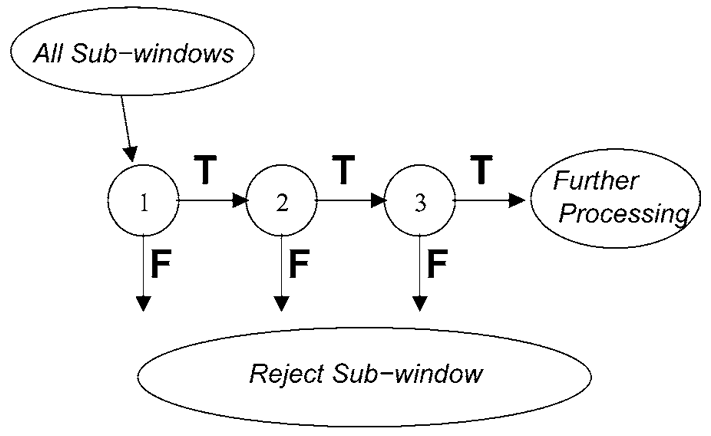
\includegraphics[width=0.4\textwidth]{process.png}
\caption{检测过程的示意图. 一系列分类器应用到每一个子区域上, 最开始的分类器用很少的处理过程便淘汰了很多负样例, 接下去的分类器用更多的计算淘汰其他的负样例. 经过多层计算以后子区域的数量急剧减少. 进一步的处理可以使用级联的另一些层 (正如我们的系统所采用的) 或者其他的检测系统.}
\label{fig:process}
\end{figure}

\subsection{训练级联分类器}\label{sec:train_cascade}
级联的设计过程受检测和性能目标驱动. 对于面部检测任务, 过去的系统已经有了很好的检测率 (大约是$85\%-95\%$) 和极低的误报率 (在$10^{-5}-10^{-6}$的数量级). 级联层的数量和每层的大小必须足够以便能够达到相似的检测性能并减少计算.

对于一个训练过的级联分类器, 它的误报率是
\[
F=\prod_{i=1}^{K}f_i
\]
其中$F$是级联分类器的误报率, $K$是分类器的数量, $f_i$是第$i$个分类器在通过它的样例上的误报率. 检测率是
\[
    D=\prod_{i=1}^{K}d_i
\]
其中$D$是级联分类器的检测率, $K$是分类器的数量, $d_i$是第$i$个分类器在通过它的样例上的检测率.

若给定整体的误报率和检测率的具体目标, 在检测过程中每一层的目标比率便能够确定下来. 比如对于一个$10$层的分类器, 若要达到$0.9$的检测率, 只要每一层有$0.99$的检测率即可 (因为$0.9\approx0.99^{10}$). 尽管这个目标检测率听起来令人气馁, 实际上很简单. 每一层的误报率只要限制在$30\%$左右即可 ($0.30^{10}\approx6\times10^{-6}$).

扫描实际图像时评估的特征数量是一个概率过程. 任何一个给定的子区域将沿级联结构向下传播, 每次一个分类器, 直到能够决定它是一个负例. 在很少的情况下, 这个区域能够通过每一个测试, 最终被标注为正例. 这个过程的行为由典型测试集中图像区域的分布决定. 每一个分类器性能的主要量度就是它的阳性率. 即被标注为可能有面部的窗口比例. 被评估特征的期望数量为
\[
N=n_0+\sum_{i=1}^{K}\left(n_i\prod_{j<i}p_j\right)
\]
其中$N$是被评估特征的期望数量, $K$是分类器的数量, $p_i$是第$i$个分类器的阳性率, $n_i$是第$i$个分类器的特征数量. 有趣的是, 因为面部非常稀少, 但是阳性率几乎和误报率相同.

级联中元素的训练过程有几个注意点. 在章节\ref{sec:learning}中呈现的 AdaBoost 学习过程仅仅尝试最小化误差, 并没有设计成以高误报率为代价得到高检测率. 均衡这些误差的一个简单和传统的方式就是调整 AdaBoost算法产生的感知器的阈值. 高阈值导致分类器有更低的误报率和更低的检测率. 更低的阈值导致更多的误报和更高的检测率. 这时不能确定若用这种方式调整阈值, AdaBoost 对训练和泛化的保证是否仍然被满足.

整个训练过程包含两种权衡. 在大多数情况中带有更多特征的分类器有着更高的检测率和更低的误报率. 与此同时, 它的计算也需要更多时间. 理论上能够得到一个最优的架构, 其中
\begin{itemize}
\item 分类器层数
\item 特征数量, 第$i$层为$n_i$
\item 每层的阈值
\end{itemize}
这些值能够被均衡, 使得在达到目标比率$F$和$D$的同时最小化特征数量. 很不幸, 这个最优化是一个极端困难的问题.
在实践中, 一个简单的架构被用来产生一个高效的分类器. 用户选择最大可接受比率$f_i$以及最小可接受比率$d_i$. 级联的每一层使用 AdaBoost 训练 (图\ref{fig:adaboost}). 在训练过程中, 被使用的特征数量不断增多, 直到检测率以及误报率达到所要的水准. 比率通过在验证集上测试得到. 如果当前整体的误报率仍然没有达到要求, 那么另一层被加到级联结构中. 训练接下去的层所用的反例收集自所有被当前检测器的误报的图像. 这些图像都是没有任何面部区域的. 这个算法在图\ref{fig:train}中被精确的描述.
\begin{figure}[!htb]
  \caption{构建级联检测器的训练算法}
  \label{fig:train}
  \kaishu\zihao{5}
  \begin{itemize}
  \item 用户选择每一层的最大可接受误报率$f$以及最小可接受检测率$d$.
  \item 用户选择最终总体误报率$F_{target}$.
  \item $P=$正例集合
  \item $N=$反例集合
  \item $F_0=1.0;\;D_0=1.0$
  \item while $F_i>F_{target}$
    \begin{itemize}
    \item $i\leftarrow i+1$
    \item $n_i=0;\;F_i=F_{i-1}$
    \item while $F_i>f\times F_{i-1}$
      \begin{itemize}
      \item $n_i\leftarrow n_i+1$
      \item 通过 AdaBoost 算法使用$P$和$N$以及$n_i$个特征训练一个分类器
      \item 用验证集评估当前级联的分类器以决定$F_i$和$D_i$的值
      \item 减小第$i$个分类器的阈值直到当前级联分类器的检测率至少为$d\times D_{i-1}$ (这也影响了$F_i$)
      \end{itemize}
    \item $N\leftarrow\varnothing$
    \item 如果$F_i>F_{target}$, 在无脸图像集合上评估当前级联检测器, 将所有误报的图像放到集合$N$中.
    \end{itemize}
\end{itemize}
\end{figure}
\subsection{简单实验}
为了检测级联方法的可行性, 我们训练了两个简单的检测器: 一个庞大的有$200$个特征的分类器, 以及一个十个有$20$个特征的分类器组成的级联结构. 级联结构中的第一层用$5000$张脸以及$10000$个从无脸图像中随机选取的非脸子区域.
第二层分类器用同样的$5000$张脸以及第一层分类器误报的$5000$个反例训练. 这个过程不断持续, 下面一层用之前层误报的反例训练.

有$200$个特征的分类器用所有训练级联分类器的样例训练. 注意到不像级联分类器, 我们很难选择无脸样例来训练那个庞大的分类器. 我们当然可以从我们所有的无脸图像中选择所有可能的子区域, 但是这让训练时间变得非常长, 不具有可操作性. 级联分类器训练的连续性大大减少了无脸的训练集. 它丢弃了简单的样例, 只留下了比较困难的那一些.

图\ref{fig:comp}展示了这两种分类器性能的$ROC$曲线. 可以看出在精确度上这两者区别不大, 但是在速度上却有很大差异. 级联分类器比另一个快了将近$10$倍, 因为它的第一层便丢弃了大多数的无脸区域, 那些便不再被后续层评估.
\begin{figure}
\centering
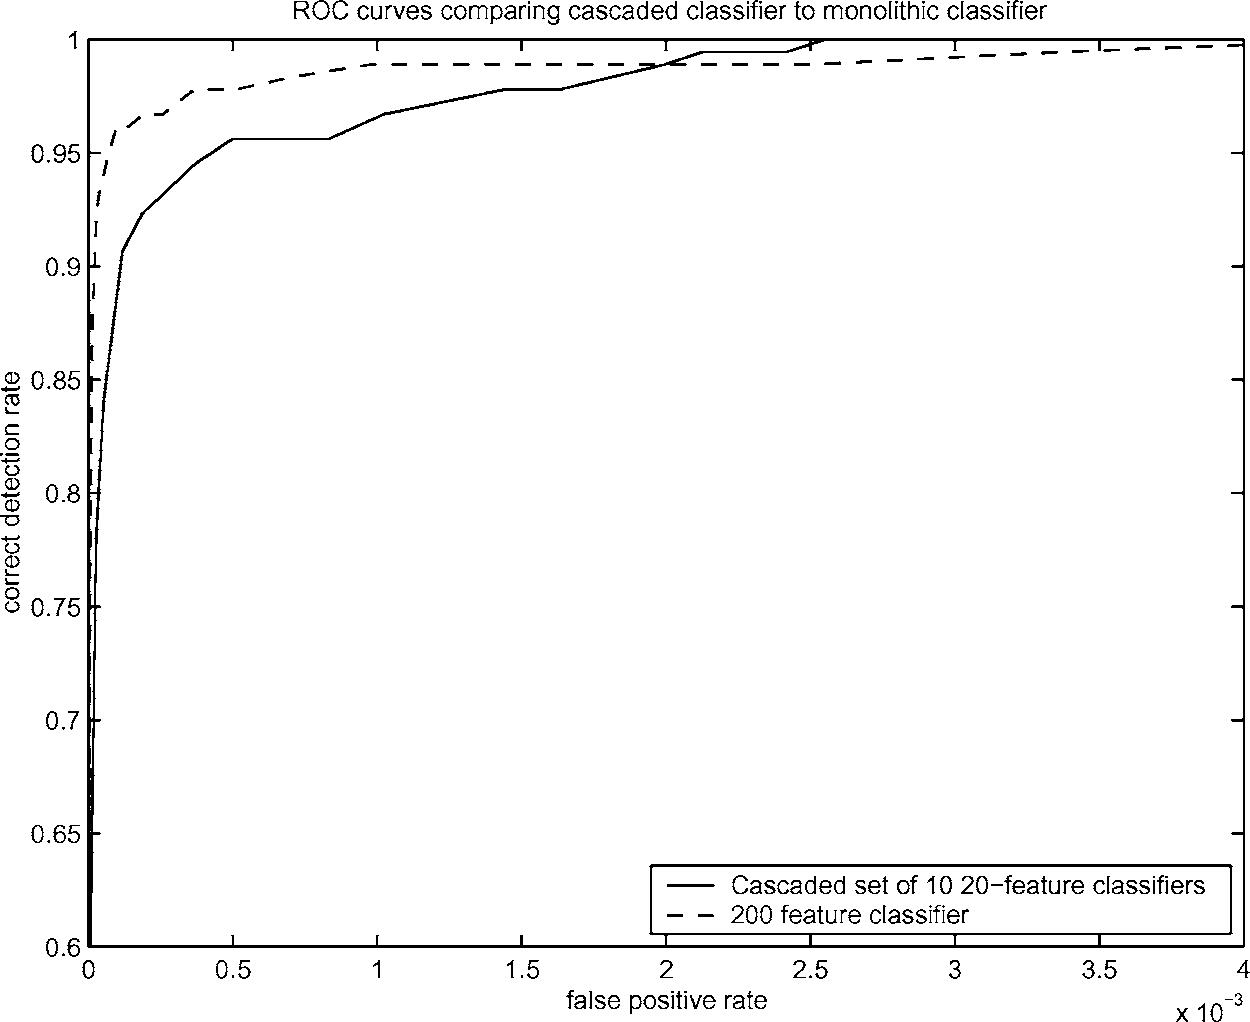
\includegraphics[width=0.4\textwidth]{ROC.png}
\caption{两种分类器的 ROC 曲线. 准确度上没有很大的差异, 但是级联检测器的检测速度快了将近$10$倍.}
\label{fig:comp}
\end{figure}
\subsection{对级联检测器的讨论}
把检测器当作一系列分类器来训练有一个隐藏的好处, 那便是最终的检测器能够看到很多负样本. 可以想象为了训练一个带有很多特征的分类器, 我们不得不通过观察特征的部分和, 当它低于某个阈值的时候便停止计算, 以此来加快运行速度. 这种方式的一个缺陷就是为了能看到训练结果, 负样本的训练集不得不变得很小 (差不多$10000-100000$个样例).
在级联检测中, 最终层为了找到先前层中失败的$10000$个负样例不得不搜寻成百上千万个负样例. 所以负训练集变得更大, 而且级联检测器能够更聚焦于困难的样例.

和级联相似的想法出现在\citet{rowley1998neural}中的面部检测系统中. 他训练了两个神经网络. 一个神经网络复杂性适当, 聚焦于图像的小部分区域, 面部检测误报率比较低. 另外一个神经网络更快, 聚焦于图像更大的区域, 面部检测误报率较高. 第二个较快的网络被用来预筛选图像, 为慢而精确的网络找到候选区域.
尽管很难准确地判定, 看上去这两个神经网络是现存最快的面部检测器\footnote{在其他已公布的面部检测系统中可能有更快的. 这些系统要么忽略了对性能的详细讨论, 要么从未公布在一个大而困难的训练集上的检测率以及误报率}. 我们的系统使用了一个类似的方法, 但是将它的两层结构拓展为$38$层级联结构.

级联检测过程的结构就是一个蜕化决策树, 这和\citet{amit1999computational}的工作相关. 不像那些使用固定检测器的技术, 他们提出了一个另类的想法. 他们使用不寻常的共同出现的简单图像特征触发更复杂的检测过程.
通过这种方式整个检测过程不需要在那么多可能图像位置和大小上进行评估. 尽管这种想法非常有价值, 但是在他们的实现中仍然需要在每一个位置事先进行一些特征检测. 这些特征之后被组合起来去发现不常见的共同出现的特征. 因为我们的检测器和使用的特征非常高效, 在每一个尺寸和位置上评估我们的检测器的花费分摊后比在图像中寻找并组合边缘快多了.

在最近的工作中,\citet{fleuret2001coarse}展示了一个面部检测技术. 它依赖一个测试链标识出特定尺寸和位置上出现的面部. 他们检测的图像属性分析出了良好的尺寸边缘特征, 这和矩形特征完全不同. 矩形特征存在于所有的尺寸中, 简单而可以被解释. 这两种方式在学习思路上也完全不同.
因为 Fleuret 和 Geman 的学习过程没有使用负样例, 他们的方法更多的基于密度估计, 相对的我们的检测器纯粹的是图像判别. 最终他们的方法检测出的误报率比之前\citet{rowley1998neural}的方法以及这个方法更高. 在已发布的论文中包括的样例图上, 每一个都有$2-10$个的误报数. 在很多实际任务中, 任何图像上的误报期望数量必须保持在一个以下 (当然在很多任务中命中数量也在一个以下). 很不幸, 论文中并没有报告在标准数据集上的检测数量以及误报的结果.
\section{结果}\label{sec:result}
这个章节描述了最终的面部检测系统. 我们讨论了系统结构的细节, 级联检测器的训练以及在一个真实的大测试集上的结果.
\subsection{训练数据集}
面部训练集由$4916$张手工标注的图, 每一张图都被放缩到$24\times24$的基准分辨率并对准. 这些脸都是通过万维网爬虫随机抓取的图像中截取的. 一些经典的面部样例展示在图\ref{fig:face_used}中. 这些训练集中的脸只是大略对准. 一个框放在人脸上, 略高于眉毛, 下边则大致在嘴和下颚之间, 然后将框放大$50\%$, 之后便截取下来放缩到$24\times24$. 我们没有做进一步的对准, 比如眼睛就没有对准. 注意到这些样例比\citet{rowley1998neural}或者\citet{sung1998example}使用的图有更多脸部部分. 最初的实验也使用了$16\times16$的训练图, 这些图里脸被截掉得更多, 但得到了只差一点点的结果. 据猜测, $24\times24$的版本包含了额外的视觉信息, 像下颚, 脸以及发际线的轮廓. 这些信息帮助我们提高了准确度. 因为被使用特征的性质, 更大尺寸的子区域并没有降低性能. 事实上, 更大的子区域中包含的额外信息能够让非脸部区域在级联检测过程中更快地被拒绝.
\begin{figure}
\centering
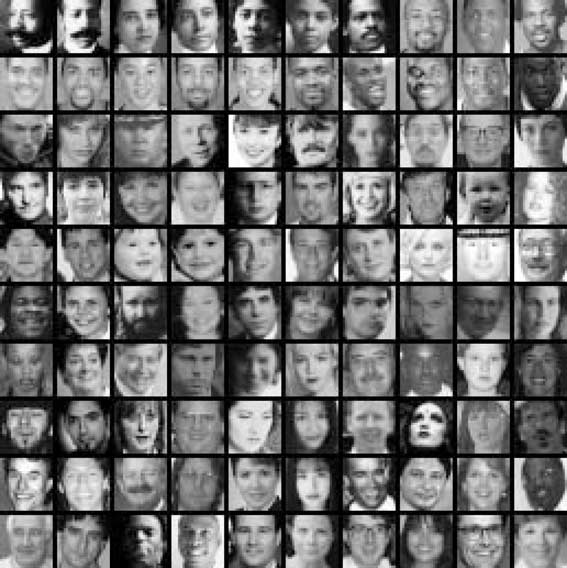
\includegraphics[width=0.4\textwidth]{face_used.png}
\caption{训练用的直立正脸样例}
\label{fig:face_used}
\end{figure}
\subsection{级联检测器的结构}
最终的检测器级联了$38$层的分类器, 里面总共包含了$6060$个特征.

在级联中的第一个分类器使用了两个特征, 拒绝了大约$50\%$的非脸区域, 同时正确检测了将近$100\%$的脸. 下一个分类器有$10$个特征, 拒绝了$80\%$的非脸区域, 同时检测出几乎$100\%$的脸.
接下去的两层都是有$25$个特征的分类器, 再接下去是有$50$个特征的分类器, 以此往后是一些依据图\ref{fig:train}中的算法选取的不同数量特征的分类器. 每一层特征数量的选取由试错过程决定. 我们不断增加特征的数量, 直到误报率急速下降. 更多的层被不断添加进来, 直到验证集上的误报率接近$0$的同时保持一个较高的正确检测率. 最终层数以及每层的大小对于最终系统的性能而言不是最重要的.
为了减少检测器的训练时间, 我们用来选取每层特征数量的过程受人干预 (针对开始的$7$层). 同样因为减轻计算的压力, 我们轻微地修改了图\ref{fig:train}中描述的算法. 我们显式地指定了每层特征的最小数量, 每次添加不止一个的特征. 在后面的层中, 在验证集上测试前我们每次添加$25$个特征.
这种方法避免了每次添加一个特征后都得在验证集上测试一次的情况.

被用来训练级联第一级的非脸部子区域是从$9500$张不包含脸的图像中随机选取的. 接下去几层使用的非脸部训练样例来自于用部分级联扫描大的非脸部图像得到的误报样例. 对于每一层, 我们收集了最多有$6000$个像这样的非脸部子区域. 在$9500$张非脸部图像中包含了大约$3.5$亿个非脸部子区域.

整个$38$层检测器的训练时间在一台$446$MHz AlphaStation XP900 机器上需要数周. 我们已经将算法并行化, 现在它能够在大约一天以内训练出一个完整的级联结构.

\subsection{最终检测器的速度}
级联检测器的速度和扫描每个子区域评估的特征数量直接相关. 正如章节\ref{sec:train_cascade}所述, 被评估的特征数量依赖于扫描的图像. 因为大量的子区域在级联的前两个阶段就被丢弃, 在$6060$个样例中平均每个子区域需要计算大约$8$个特征 (计算于 MIT + CMU\citep{rowley1998neural}). 在一个 $700$Mhz Pentium $\RN{3}$处理器上, 面部检测器能在$0.067$秒内处理一张$384\times288$像素的图像. 它以$1.25$的开始尺寸以及$1.5$的步长扫描). 这个速度比 Rowley-Baluja-Kanade 检测器\citep{rowley1998neural}快了大约$15$倍, 比Schneiderman-Kanade 检测器\citet{schneiderman2000statistical}快了大约$600$倍.

\subsection{图像处理}
为了最小化不同光照条件的影响, 训练中所有样例的子区域方差都被规范化. 因此在检测过程中规范化也是必须的. 一张图像的子区域方差能够通过积分图很快地计算出来. 在公式$\sigma^2=m^2-\frac1N\sum x^2$中, $\sigma$代表标准差, $m$是均值, $x$则是子区域中的像素值. 子区域的均值能够通过积分图计算出来. 像素平方之和能够通过像素平方后图像的积分图计算出来 (在扫描过程中使用了两张积分图).
在扫描过程中图像规范化能够在乘上特征值后进行而不是直接在像素上操作.

\subsection{检测器的扫描过程}
最终的检测器在多个尺寸和位置对图像进行扫描. 我们放缩检测器自己而不是放缩图像. 因为在任何尺寸上面的特征评估需要的时间是一定的, 所以这个过程才有意义. 当放缩倍数为$1.25$时我们得到了较好的检测结果.

检测器也在不同位置进行扫描. 我们通过移动窗口$\Delta$数量像素的距离来到达一系列位置. 移动过程收到检测器尺寸的影响: 如果当前尺寸为$s$, 窗口就移动$[s\Delta]$, 这里$[]$代表四舍五入的操作.

$\Delta$的选择同时影响着检测速度以及准确度. 因为训练图有一些平移变易性, 尽管在图像中只移动了小距离, 学得的检测器仍然能获得良好的检测性能. 因此检测的子区域一次能够平移多个像素.
然而, 多个像素的步长会略微减小检测率, 与此同时误报数也会减少. 我们展示了两种不同步长的结果.

\subsection{多检测器的融合}
因为最终的检测器对平移和尺寸的微小变化并不敏感, 在一张扫描图像中对每张脸常常会进行多次检测. 这对于某些误报类型也正确. 实践中对每张脸返回一个最终结果的做法通常是很有意义的. 在这之后对检测的子区域进行后期处理以将这些重叠的检测合并成一次检测.

在这些实验中检测结果以一种很简单的方式合并. 检测结果集首先被分割成不相交的子集. 如果两个检测结果的边界有重叠, 它们便在同一个集合中. 每个划分就产生了一个最终的检测结果. 最终边界的拐角就是集合中所有拐角的平均值.

在某些情况中, 这个后期处理减少了误报的数量, 因为误报的重叠子集被合并成一个检测结果了.
\subsection{真实测试集上的实验}
我们在MIT + CMU 前端界面测试了我们的系统\citep{rowley1998neural}. 这个集合包含了$130$张图片, 其中有$507$张被标记的正脸. 图\ref{fig:step_dif}中展现了一条ROC曲线, 它展示了我们检测器的性能. 为了创建这条 ROC 曲线, 分类器的最终层感知器的阈值在$-\infty$和$+\infty$之间调整. 
\begin{figure}[!b]
\centering
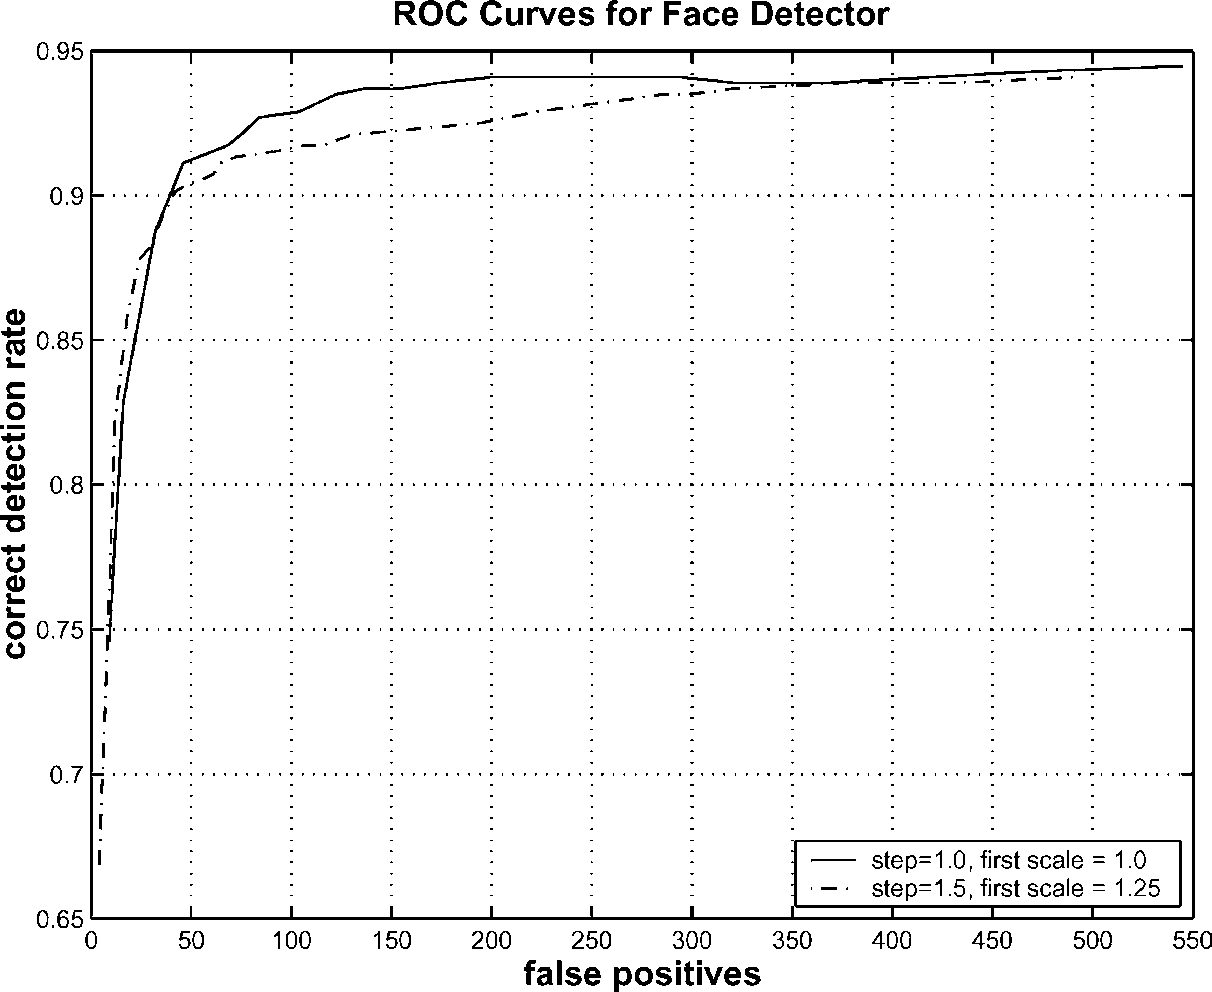
\includegraphics[width=0.4\textwidth]{step_dif.png}
\caption{我们的面部检测器在 MIT + CMU 测试集上的 ROC 曲线. 第一次使用了$1.0$的步长, $1.0$初始尺寸, 扫描了$75081800$个子区域. 第二次使用了$1.5$的步长, $1.25$初始尺寸, 扫描了$18901947$个子区域. 两者的放缩因子都是$1.25$}
\label{fig:step_dif}
\end{figure}
调整阈值到$+\infty$将导致检测率和误报率降到$0$, 调到$-\infty$则会同时提高检测率和误报率, 但止于一个特定点. 没有一个比率能够高于除去最终层的级联的比率.
事实上, 一个$-\infty$的阈值等价于将层移除. 进一步提高检测率和误报率需要减少级联中下一层分类器的阈值. 因此, 为了构造出一个完整的 ROC 曲线, 分类器层被不断移除.
我们使用误报的数量而不是误报率作为 ROC 曲线的$x$坐标. 这有助于和其他系统进行比较. 计算误报率时, 简单地除以扫描的子区域总数即可.
当$\Delta=1.0$, 开始的放缩比率为$1.0$, 扫描的子区域总数为$75081800$. 当$\Delta=1.5$, 开始的放缩比率为$1.25$时, 扫描的子区域总数为$18901947$.

不幸的是, 之前公布的大多数面部检测结果仅仅包括了一个单一的操作规程, 在 ROC 曲线上只有一个点.
为了更容易地和我们的检测器进行对比, 我们列举了当误报率相同时不同系统报告的检测率. 表\ref{tab:false}展现了我们以及其他系统在不同误报数量下的检测率. 根据Rowley Baluja-Kanade 的结果\citep{rowley1998neural}, 他们不同版本的检测器测试出了不同的结果.
\begin{table}
\centering
\begin{tabular}{lcccccccc}
\firsthline
&\multicolumn{8}{c}{误报率} \\
\cline{2-9}
检测器 & 10 & 31 & 50 & 65 & 78 & 95 & 167 & 422 \\
\hline
Viola-Jones & $76.1\%$ & $88.4\%$ & $91.4\%$ & $92.0\%$ & $92.1\%$ & $92.9\%$ & $93.9\%$ & $94.1\%$ \\
Viola-Jones (voting) & $81.1\%$ & $89.7\%$ & $92.1\%$ & $93.1\%$ & $93.1\%$ & $93.2\%$ & $93.7\%$ & - \\
Rowley-Baluja-Kanade & $83.2\%$ & $86.0\%$ & - & - & - & $89.2\%$ & $90.1\%$ & $89.9\%$ \\
Schneiderman-Kanade & - & - & - & $94.4\%$ & - & - & - & - \\
Roth-Yang-Ahuja & - & - & - & - & ($94.8\%$) & - & - & - \\
\lasthline
\end{tabular}
\caption{不同误报数下的检测率. 测试集为 MIT + CMU, $130$张图, $507$个人脸}
\label{tab:false}
\end{table}
尽管对于特定的检测器, 这些结果并不能正确地标注在 ROC 曲线上, 他们转而公布了一系列这个系统能够达到的性能点. 他们确实公布了两个检测器的 ROC 曲线, 但是这些曲线并不能代表他们最好的结果. 
对于 Roth-Yang-Ahuja 的检测器\citep{yang2000snow}, 他们报告了 MIT + CMU 测试集上的检测结果. 这个测试集中他们除去了五张脸上有线的图, 因此测试集只包含了$125$张图, $483$张脸. 想必在整个测试集上他们的检测率会更低. 表中他们检测率两边的括号表明了他们略微不同的测试集.
Sung 和 Poggio 的面部检测器\citep{sung1998example}在 MIT 上进行了测试, 因为那时候 CMU 部分还不存在. MIT 测试集上包含了$23$张图, $149$张脸. 他们获得了$79.9\%$的检测率以及$5$个误报. 我们在 MIT 上的检测率则是$77.8\%$, 有$5$个误报.

图\ref{fig:output}中展现了我们的系统在 MIT + CMU 测试集中部分图像上的测试结果.
\begin{figure}[!b]
\centering
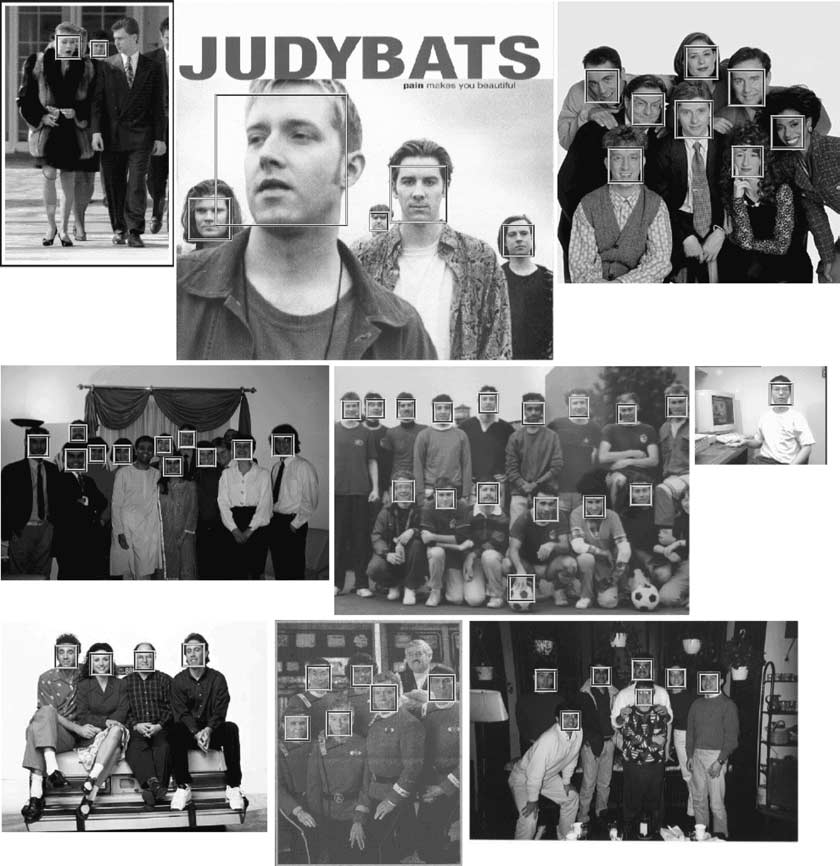
\includegraphics[width=0.6\textwidth]{output.png}
\caption{面部检测器在 MIT + CMU 测试集上的部分输出结果}
\label{fig:output}
\end{figure}
\subsection{简单投票机制提高检测结果}
可以通过联合这三个检测器得到一个最好的结果. 这三个检测器的训练采用了不同初始负样本, 略微不同的正负误差权重, 为分类器大小以及误报数制定了不同的权衡策略. 在最终的任务中, 这三个系统有相似的表现, 但是在某些情况下他们的错误是不同的. 因此我们采取如下方法来将他们的结果合并: 当且仅当通过至少两个检测器时, 该结果才被保留. 这个方法提高了检测率, 淘汰了更多的误报结果. 因为他们的检测错误是无关联的, 所以他们联合起来的结果比单一一个检测器有了极大的提升.

\subsection{失败模式}
通过观察我们的检测器在多个测试集上的评测结果后, 我们发现了一些失败模式.

面部检测器是用正面右上角的脸进行训练的. 这些测试集中的脸只是被粗略地校准, 因此, 在图片平面内外都存在一些旋转角度. 经过正式的观察和分析, 我们发现只有当脸在平面内旋转角度$\pm\ang{15}$内, 平面外旋转角度$\pm\ang{45}$内才能被正确检测 (通过一个剖面图视角). 超出上述范围这个检测器就不能正确检测了.

我们也注意到刺眼的背景光也会导致检测失败. 这种情况下脸变得非常暗, 同时背景却相对比较亮. 有趣的是当我们用鲁棒的估计算法进行非线性方差正规化后, 去除极端值的同时检测率也提高了不少. 然而在我们的系统中加入这个正规化后增加了非常多的计算量.

最后, 我们的检测器失效于那些重要部位被挡住的脸. 例如如果眼部被挡住, 检测器就经常失效. 嘴部并不是很重要, 所以一张挡住嘴的脸仍然能够被检测出来.

\section{结论}\label{sec:discussion}
我们已经展示了面部检测方法, 它最小化了计算时间, 达到了非常高的检测精度. 这个方法被用来构造一个面部检测系统, 它比之前其他方法快了将近$15$倍. 我们进行了初步的实验, 并在其他地方进行了详细说明. 实验结果显示, 其他物体的高效检测器, 比如行人以及摩托车等也可以通过这种方式构造出来.

这篇论文将新的算法, 新的表示方法, 新的观点结合在一起, 形成了一个非常通用的方法. 这将被更加广泛地应用于计算机视觉以及图像处理中.

我们的第一个贡献是是用积分图计算巨大的图像特征集合. 这是一个新的技术. 为了得到真正的尺寸不变性, 几乎所有的面部检测系统必须在不同的图像尺寸上进行操作. 积分图淘汰了这种计算金字塔状多尺寸图像的需求, 极大地减少了面部检测系统需要的初始图像处理流程, 同时能够以几乎同样的时间完成计算.

与此同时, 积分图也能立即用在那些使用类哈尔特征的系统上, 比如\citet{papageorgiou1998general}. 可以预见, 这将对那些利用类哈尔特征的任务产生一定的影响. 初步的实验也显示一个类似的特征集合在参数模拟任务中也表现得十分高效. 在这类任务中, 我们需要决定人脸的表情, 头的位置, 或者物体的姿态.

第二个贡献就是利用 AdaBoost 特征选取算法选取计算高效的特征, 并在这个特征的基础上构建一个简单高效的分类器. 很显然这个分类器对于面部检测来说十分高效, 我们也坚信它在其他领域中也能保持高效性, 比如摩托车和行人识别. 更进一步的是, 我们在特征选取中采用的积极而高效的技术手段将对大量的学习任务产生影响. 若有了一个高效的特征选取工具, 系统设计师就能够更加自由地把非常大非常复杂的特征集合作为学习过程的输入数据.
最终的分类器计算仍然十分高效, 因为在运行的时候只有一小部分的特征需要被计算. 分类器往往非常简单, 在一个复杂特征的巨大集合里, 往往能够找到一些至关重要的特征. 那些特征能够以一种直接的方式捕捉到分类问题的内在结构.

这篇论文的第三个贡献就是构造了一个级联分类器, 它能急剧减少计算时间, 提高检测精度. 级联结构的早期阶段被设计成拒绝大部分图像, 将后续的处理流程聚焦在更有希望的区域上. 一个关键点就是展现出的级联层在结构上都是简单和相同的.
先前采用的细致过滤的方法, 比如\citet{itti1998model}, 提出了一个更加复杂和成分混杂的机制. 类似的,\citet{amit1999computational}提出了一个分级的检测结构, 但是各级的结构和处理方式上完全不同. 一个同质的系统, 在实现和理解上比较简单, 同时能够在处理时间和检测性能之间进行简单的权衡.

最后这篇论文详尽地描述了一些实验. 这些实验采用了一个困难的且被广泛研究的面部检测数据集. 这个数据集中包括了很多种状况下的脸: 不同的照明条件, 不同尺寸, 不同姿态, 不同的照像机等. 在这样子庞大而复杂的数据集上进行实验是非常困难和耗时的. 然而, 能够在这类条件下工作的系统不太可能不稳定, 也不太可能只限制在某些特殊条件下. 更重要的是, 从这个数据集上得到的结论不可能是实验假像.
\section{致谢}
作者们对 T.M. Murali, Jim Rehg, Tat-Jen Cham, Rahul Sukthankar, Vladimir Pavlovic 和 Thomas Leung 提出的帮助性建议表示感谢. 同时我们也非常感谢 Henry Rowley 提供的面部检测器实现, 让我们能够进行充分的比较.
\bibliography{reference}
\end{document}
